
\documentclass[journal,onecolumn]{IEEEtran}

\usepackage{cite}
\usepackage{amsmath,amssymb,amsfonts}
\usepackage{graphicx}
\usepackage{booktabs}
\usepackage{array}
\usepackage{multirow}
\usepackage{longtable}   % contribution table: not a float, may break across pages
\usepackage{xcolor}
\usepackage{textcomp}
\usepackage{tikz}
\usetikzlibrary{shapes.geometric, arrows.meta,positioning,calc,fit,backgrounds}
\usepackage{url}
\usepackage[hidelinks]{hyperref}   % keep hyperref last

\graphicspath{{figures/}}
\renewcommand{\arraystretch}{1.0}
\newcolumntype{C}[1]{>{\centering\arraybackslash}p{#1}}

\newcommand{\celebdf}{Celeb-DF}
\newcommand{\ffpp}{FF\texttt{++}}
\newcommand{\dfdc}{DFDC}
\newcommand{\best}[1]{\textbf{#1}}

\newcommand{\yes}{\ensuremath{\checkmark}}
\newcommand{\no}{\ensuremath{\times}}
\newcommand{\nm}{\textit{\footnotesize n/m}}

\setlength{\textfloatsep}{6pt plus 2pt minus 2pt}
\setlength{\intextsep}{6pt plus 2pt minus 2pt}
\setlength{\abovecaptionskip}{4pt}
\setlength{\belowcaptionskip}{2pt}

\renewcommand{\topfraction}{0.92}
\renewcommand{\bottomfraction}{0.85}
\renewcommand{\textfraction}{0.07}
\renewcommand{\floatpagefraction}{0.75}
\setcounter{topnumber}{3}
\setcounter{bottomnumber}{2}
\setcounter{totalnumber}{4}

\begin{document}

\title{Cross-Dataset Generalization and Robustness of Deepfake Detection:\\
A Leave-One-Out Study with Explainability and Statistical Validation}

\author{%
  Kawser Sikder
  and Tasneem Abdullah Aurnobb
  \thanks{This report is submitted in partial fulfillment of the requirements of
  CSE~499A, Senior Design Project~I, Department of Electrical and Computer
  Engineering, North South University, Dhaka, Bangladesh.}%
  \thanks{Manuscript submitted September~9, 2026.}%
}

\maketitle

\begin{abstract}
Currently, artificially generated content and face manipulation have become
very common, and they are very good at producing human-like content that's hard
to distinguish from a normal person's perspective. But sadly, the detectors
that can differentiate between artificially generated and human-generated content
have not yet been upgraded to that level. The main reason most detectors fail
on today's content is that they were initially trained on a single corpus, and
their benchmarks are set by that corpus. But when the corpus changes, they fail
miserably. There is another issue with the train-test split when splitting in
frames: frames from the same video or image end up in both the training and
test sets, resulting in a leak, and as a result, the benchmark number is no
longer authentic. Three public datasets, Celeb-DF v2, FaceForensics++, and
DFDC, containing manipulated face videos, have been combined. To avoid data
leakage that had previously inflated the results, the data has been split into
training and testing sets based on subject identity rather than on individual
frames. The detector is evaluated within each dataset, across all ordered
pairs, and with a leave-one-out approach. In this approach, two datasets are
used for training, while the third, unseen dataset, is used for testing. Out-of-domain
Grad-CAM maps show 26.5--39.3\% higher border energy while entropy
decreases, so attention is drawn to the wrong
region, and the model's confidence provides no warning of this failure. JPEG
q10 reduces Celeb-DF AUC from 0.7579 to 0.5342
(13.3\% of above-chance discrimination retained). Compression-aware training
recovers 52.6\% at a clean cost of $-$0.0006, but
does not transfer to unseen corruptions. Wider augmentation yields only two
significant gains and one significant loss across 15 unseen comparisons, with
the gains occurring only in cases where the corruption shares a physical
mechanism with the added training families.
The greatest gain comes from training-dataset diversity ($+0.280$ to $+0.305$
from more videos against $+0.066$ of an ensemble). On FaceForensics++, 0.8788
is reached with a dual RGB-DCT stream, while domain-adversarial training and
Grad-CAM supervision lose 0.031 and 0.006, respectively. For latent-diffusion
edits, the median AUC is 0.480, and of the nine checkpoints, four ranked
forgeries as more authentic than their real sources. Overall, generalization is
more related to a broader training set and stable manipulation cues than to
simply adding more types of corruption.
\end{abstract}

\begin{IEEEkeywords}
Convolutional neural networks, cross-dataset generalisation, data augmentation,
deepfake detection, explainable artificial intelligence, image forensics, model
robustness, statistical validation.
\end{IEEEkeywords}

\section{Introduction}
\label{sec:intro}

Face manipulation using deepfakes has become cheap and accessible. Convincing fake videos can be produced using publicly available software and a single GPU from only a small number of photographs, creating risks such as non-consensual imagery, financial fraud, and political disinformation. Detection systems can achieve more than 99\% accuracy on standard benchmarks, but these results often do not represent their performance outside the training conditions. A detector also needs to handle an unseen manipulation method, a generation tool that did not exist during training, and platforms that re-encode uploaded media. We selected this problem because there is a large gap between benchmark performance and deployment performance, this gap is poorly documented, and it can be studied using undergraduate computing resources. Our objectives are to measure cross-dataset transfer, explain why generalization fails, and test whether common robustness methods work under unseen conditions.

We evaluate three public corpora: \celebdf~(v2), FaceForensics\texttt{++}, and the Deepfake Detection Challenge (DFDC) sample, providing 229\,977 face crops from 8\,909 videos~\cite{li2020celebdf,rossler2019faceforensics,dolhansky2020dfdc}. \celebdf{} provides higher-quality manipulated faces, FaceForensics\texttt{++} is a widely used benchmark with known source relationships, and DFDC adds a different data and compression profile. We keep preprocessing minimal. The face crops are resized to $224 \times 224$ and normalized using ImageNet statistics. The key step is structural. Each frame is mapped to its video ID, and FaceForensics\texttt{++} videos that share a source identity are merged using union--find before the data is split. This prevents near-duplicate frames and shared identities from appearing across the train--test boundary and inflating performance. The FF\texttt{++} dataset also has a single-manipulation-method limitation that should be considered when interpreting its in-domain results.

The literature mainly follows three directions. R{\"o}ssler \textit{et al.} introduced FaceForensics\texttt{++} and showed that XceptionNet~\cite{chollet2017xception} achieves high in-domain performance but decreases in performance as image quality becomes lower~\cite{rossler2019faceforensics}. Li \textit{et al.} later showed that detectors scoring above 0.98 on earlier datasets dropped to around 0.65 on \celebdf{}~\cite{li2020celebdf}. Other studies focus on generalization through different representations or training signals. Qian \textit{et al.} explored frequency-domain clues~\cite{qian2020f3net}, Haliassos \textit{et al.} used temporal mouth dynamics and reported 0.824 on unseen \celebdf{}~\cite{haliassos2021lips}, while Shiohara and Yamasaki used self-blended images and reached 0.932 in their reported setting~\cite{shiohara2022sbi}. From a methodological perspective, Yan \textit{et al.} showed that conclusions can change under a unified evaluation protocol~\cite{yan2023deepfakebench}, while Hendrycks and Dietterich established the corruption framework that we adapt here to test robustness against corruption types withheld from training~\cite{hendrycks2019robustness}.

These studies leave five gaps that can hide failure. Cross-dataset transfer is usually reported pairwise, leaving the more difficult leave-one-out setting less explored. Robustness and generalization are also often studied separately, even though deployment may involve both at the same time. Corruption tests commonly use the same corruption families seen during training, making it difficult to separate memorization from actual robustness. Point estimates without confidence intervals can also make small differences appear meaningful. Finally, frame-level splits can allow the same subject or near-duplicate frames to cross the evaluation boundary.

We address these issues using a controlled protocol based on EfficientNet-B0~\cite{tan2019efficientnet}. For the main comparison, the backbone, training schedule, sampler, and seed are held fixed; the architectural experiments in Section~\ref{ssec:extensions} are treated as separate extensions rather than part of this comparison. The main study measures in-domain performance, all six ordered cross-corpus pairs, and three-way leave-one-out generalization. Grad-CAM~\cite{selvaraju2017gradcam} is reduced to three scalar measures, namely center of mass, entropy, and border energy, so that changes in attention can be tested numerically. Robustness is evaluated under recompression, blur, rescaling, and noise, using paired bootstrap intervals to compare performance on corruption types withheld from training. Section~\ref{sec:proposed} describes the system and evaluation protocol. Section~\ref{sec:results} presents cross-dataset transfer, explainability and robustness, statistical validation, data scaling, the ablation study, comparison with published work, and architectural and objective extensions. The final extension also tests latent-diffusion manipulation. None of the detectors survives this probe, and four of nine checkpoints score below chance, meaning they rank the forged images as more authentic than their real counterparts. Section~\ref{sec:conclusion} concludes the report and outlines the work for CSE~499B.

\section{Proposed System}
\label{sec:proposed}

The system is a video-level deepfake detector built on a single convolutional
backbone that was held fixed across every experiment. The pipeline appears in
Fig.~\ref{fig:flowchart} and runs in four stages: data ingestion with identity
recovery, leakage-safe splitting, frame-level training, and video-level
evaluation under clean and degraded conditions.

\begin{figure}[!ht]
\centering
\resizebox{0.72\textwidth}{!}{%
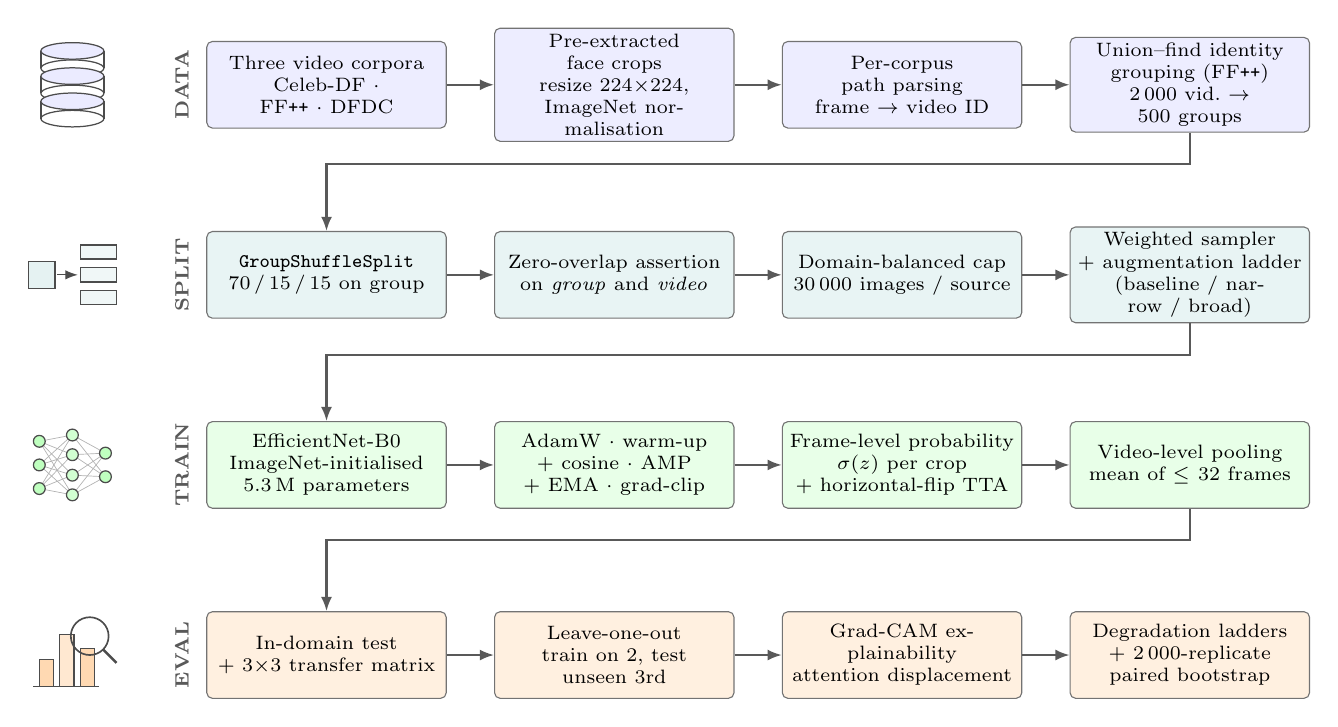
\begin{tikzpicture}[
  font=\scriptsize,
  node distance=6mm,
  box/.style   = {draw=black!55, rounded corners=2pt, align=center,
                  text width=29mm, minimum height=11mm, inner sep=2pt},
  data/.style  = {box, fill=blue!7},
  split/.style = {box, fill=teal!9},
  train/.style = {box, fill=green!9},
  eval/.style  = {box, fill=orange!12},
  arr/.style   = {-{Latex[length=1.8mm,width=1.4mm]}, thick, draw=black!65},
  lbl/.style   = {font=\scriptsize\bfseries, anchor=west, text=black!65}
]

\node[data] (a1) {Three video corpora\\ \celebdf{} $\cdot$ \ffpp{} $\cdot$ \dfdc};
\node[data, right=of a1] (a2) {Pre-extracted face crops\\ resize $224{\times}224$,\\ ImageNet normalisation};
\node[data, right=of a2] (a3) {Per-corpus path parsing\\ frame $\rightarrow$ video ID};
\node[data, right=of a3] (a4) {Union--find identity\\ grouping (\ffpp{})\\ 2\,000 vid.\ $\rightarrow$ 500 groups};

\draw[arr] (a1) -- (a2);
\draw[arr] (a2) -- (a3);
\draw[arr] (a3) -- (a4);

\node[split, below=13mm of a1] (b1) {\texttt{GroupShuffleSplit}\\ 70\,/\,15\,/\,15 on group};
\node[split, right=of b1] (b2) {Zero-overlap assertion\\ on \emph{group} and \emph{video}};
\node[split, right=of b2] (b3) {Domain-balanced cap\\ 30\,000 images / source};
\node[split, right=of b3] (b4) {Weighted sampler\\ + augmentation ladder\\ (baseline / narrow / broad)};

\draw[arr] (b1) -- (b2);
\draw[arr] (b2) -- (b3);
\draw[arr] (b3) -- (b4);
\draw[arr] (a4.south) -- ++(0,-4mm) -| (b1.north);

\node[train, below=13mm of b1] (c1) {EfficientNet-B0\\ ImageNet-initialised\\ 5.3\,M parameters};
\node[train, right=of c1] (c2) {AdamW $\cdot$ warm-up\\ + cosine $\cdot$ AMP\\ + EMA $\cdot$ grad-clip};
\node[train, right=of c2] (c3) {Frame-level probability\\ $\sigma(z)$ per crop\\ + horizontal-flip TTA};
\node[train, right=of c3] (c4) {Video-level pooling\\ mean of $\leq 32$ frames};

\draw[arr] (c1) -- (c2);
\draw[arr] (c2) -- (c3);
\draw[arr] (c3) -- (c4);
\draw[arr] (b4.south) -- ++(0,-4mm) -| (c1.north);

\node[eval, below=13mm of c1] (d1) {In-domain test\\ + $3{\times}3$ transfer matrix};
\node[eval, right=of d1] (d2) {Leave-one-out\\ train on 2, test unseen 3rd};
\node[eval, right=of d2] (d3) {Grad-CAM explainability\\ attention displacement};
\node[eval, right=of d3] (d4) {Degradation ladders\\ + 2\,000-replicate\\ paired bootstrap};

\draw[arr] (d1) -- (d2);
\draw[arr] (d2) -- (d3);
\draw[arr] (d3) -- (d4);
\draw[arr] (c4.south) -- ++(0,-4mm) -| (d1.north);

\node[lbl, left=1mm of a1.west, rotate=90, anchor=south] {DATA};
\node[lbl, left=1mm of b1.west, rotate=90, anchor=south] {SPLIT};
\node[lbl, left=1mm of c1.west, rotate=90, anchor=south] {TRAIN};
\node[lbl, left=1mm of d1.west, rotate=90, anchor=south] {EVAL};

\tikzset{ic/.style={draw=black!70, line width=0.45pt}}

\begin{scope}[shift={($(a1.west)+(-17mm,0mm)$)}]
  \foreach \dy in {3.2mm,0mm,-3.2mm}{
    \begin{scope}[shift={(0mm,\dy)}]
      \draw[ic] (-4mm,1.1mm) -- (-4mm,-1.1mm);
      \draw[ic] ( 4mm,1.1mm) -- ( 4mm,-1.1mm);
      \draw[ic] (0mm,-1.1mm) ellipse (4mm and 1.05mm);
      \draw[ic, fill=blue!8] (0mm,1.1mm) ellipse (4mm and 1.05mm);
    \end{scope}}
\end{scope}

\begin{scope}[shift={($(b1.west)+(-17mm,0mm)$)}]
  \draw[ic, fill=teal!10] (-5.6mm,-1.7mm) rectangle (-2.2mm,1.7mm);
  \draw[ic, -{Latex[length=1.6mm,width=1.2mm]}] (-1.9mm,0mm) -- (0.7mm,0mm);
  \draw[ic, fill=teal!6] (1mm, 2.0mm) rectangle (5.6mm, 3.8mm);
  \draw[ic, fill=teal!6] (1mm,-0.9mm) rectangle (5.6mm, 0.9mm);
  \draw[ic, fill=teal!6] (1mm,-3.8mm) rectangle (5.6mm,-2.0mm);
\end{scope}

\begin{scope}[shift={($(c1.west)+(-17mm,0mm)$)}]
  \foreach \a in {3mm,0mm,-3mm}
    \foreach \b in {3.8mm,1.3mm,-1.3mm,-3.8mm}
      \draw[draw=black!30, line width=0.25pt] (-4.2mm,\a) -- (0mm,\b);
  \foreach \a in {3.8mm,1.3mm,-1.3mm,-3.8mm}
    \foreach \b in {1.5mm,-1.5mm}
      \draw[draw=black!30, line width=0.25pt] (0mm,\a) -- (4.2mm,\b);
  \foreach \a in {3mm,0mm,-3mm}
    \draw[ic, fill=green!25] (-4.2mm,\a) circle[radius=0.75mm];
  \foreach \a in {3.8mm,1.3mm,-1.3mm,-3.8mm}
    \draw[ic, fill=green!18] (0mm,\a) circle[radius=0.75mm];
  \foreach \a in {1.5mm,-1.5mm}
    \draw[ic, fill=green!25] (4.2mm,\a) circle[radius=0.75mm];
\end{scope}

\begin{scope}[shift={($(d1.west)+(-17mm,0mm)$)}]
  \draw[ic] (-5mm,-4mm) -- (3.4mm,-4mm);
  \draw[ic, fill=orange!30] (-4.2mm,-4mm) rectangle (-2.4mm,-0.6mm);
  \draw[ic, fill=orange!18] (-1.6mm,-4mm) rectangle ( 0.2mm, 2.6mm);
  \draw[ic, fill=orange!30] ( 1.0mm,-4mm) rectangle ( 2.8mm, 0.8mm);
  \draw[ic, line width=0.6pt] (2.2mm,2.4mm) circle[radius=2.4mm];
  \draw[ic, line width=0.9pt] (3.9mm,0.7mm) -- (5.6mm,-1.0mm);
\end{scope}

\end{tikzpicture}}
\caption{Complete system flowchart. Each row is one stage, marked by the
icon at its left: three video corpora, the leakage-safe split, the training
and decision pipeline, and the evaluation suite. Blue denotes data ingestion
and identity recovery, green denotes training, and orange denotes evaluation.
The identity grouping stage prevents one face from appearing on both sides of
a split, collapsing 2\,000 FaceForensics\texttt{++} videos into 500 identity
groups.}
\label{fig:flowchart}
\end{figure}

\subsection{Datasets and Preprocessing}

The three corpora supply 229\,977 face crops over 8\,909 videos.
\celebdf{}~(v2)~\cite{li2020celebdf} contributes 65\,381 crops from 6\,528 videos
at 10.0 frames per video, 86.4\% forged, with a 980-video held-out split.
FaceForensics\texttt{++}~\cite{rossler2019faceforensics} contributes 39\,949
crops from 2\,000 videos at 20.0 frames per video, balanced at 50\% forged, with
a 300-video split. Those 2\,000 videos collapse to \textbf{500 identity groups}
under the union--find pass of Eq.~\eqref{eq:identity}, and splits are made on
those groups. \dfdc{}~\cite{dolhansky2020dfdc} contributes 124\,647 crops from
381 videos at 327.2 frames per video, 80.1\% forged, with only 58 test videos.

Two properties must be stated before any number is reported. The \dfdc{} portion
is the \texttt{train\_sample} subset rather than the full challenge set, and its
58-video test split is small enough that any \dfdc{}-specific interval is wide.
The FaceForensics\texttt{++} copy available to us contains a single manipulation
method, since there are exactly 1\,000 forged folders and no method name anywhere
in the directory tree, so all its figures here describe one manipulation rather
than the four-method benchmark. Photometric preprocessing is intentionally
minimal, so that the protocol rather than the pipeline is the variable under
study: every crop is resized to $224 \times 224$ and normalized channel-wise
using ImageNet statistics.

\subsection{Leakage-Safe Splitting}
\label{ssec:splitting}

Frames from one video are near-duplicates, so a per-frame split places
near-identical images on both sides of the boundary and inflates every score.
Each frame is mapped back to its source video before any split is made, and each
corpus needs its own parser because each encodes provenance differently.

FaceForensics\texttt{++} requires one further step. A forged clip in that corpus
is synthesized from two named real clips, so folder \texttt{588\_556\_crops} is
built from real videos \texttt{588\_crops} and \texttt{556\_crops}. Splitting on
video alone would let forged \texttt{588\_556} sit in the training set while real
\texttt{588} sits in the test set, which lets the network recognize the
individual rather than the manipulation. Let $V$ be the set of videos and $N(v)$
the numeric identity tokens in the name of video $v$. We take the transitive
closure of the first relation below by union--find, which collapses 2\,000 videos
into 500 identity groups, then split on those groups and assert the second
condition in every experiment,
\begin{equation}
  u \sim v \iff N(u) \cap N(v) \neq \varnothing ,
  \qquad
  \mathcal{G}(D_i) \cap \mathcal{G}(D_j) = \mathcal{V}(D_i) \cap \mathcal{V}(D_j)
  = \varnothing , \quad i \neq j,
  \label{eq:identity}
\end{equation}
where $\mathcal{G}$ and $\mathcal{V}$ return the group and video identifiers of a
split $D$.

\subsection{Network and Training Objective}

The backbone is EfficientNet-B0~\cite{tan2019efficientnet}, chosen for a
parameter budget roughly a quarter of the XceptionNet~\cite{chollet2017xception}
that dominates this literature. Activations use the swish function $x\,\sigma(x)$,
and every block carries a squeeze-and-excitation gate~\cite{hu2018senet} that
recalibrates channels
using global context,
\begin{equation}
  z_{c} = \frac{1}{HW} \sum_{i,j} U_{i,j,c},
  \qquad
  s = \sigma\!\left( W_{2}\,\mathrm{swish}(W_{1} z) \right),
  \qquad
  \tilde{U}_{:,:,c} = s_{c}\, U_{:,:,c} .
  \label{eq:se}
\end{equation}
That gate matters because it makes the network's reliance on globally distributed
texture explicit, which is what the explainability study probes. The head is a
single logit trained with class-weighted binary cross-entropy,
\begin{equation}
  \mathcal{L} = -\frac{1}{N}\sum_{i=1}^{N} w_{y_i}
  \Big[ y_i \log \sigma(z_i) + (1-y_i)\log\big(1-\sigma(z_i)\big) \Big],
  \label{eq:bce}
\end{equation}
optimised with AdamW~\cite{loshchilov2019adamw} at learning rate and weight
decay $1\times10^{-4}$, under one epoch of linear warm-up followed by cosine
annealing~\cite{loshchilov2017sgdr}. Training uses batches
of 64 at
$224 \times 224$, mixed precision, unit-norm gradient clipping, an exponential
moving average of decay 0.999, a weighted sampler, a 70/15/15 split on identity
groups, at most 12 epochs with patience 4, and seed 42. The configuration is
identical for every model in this report, so each measured difference is
attributable to the data or the augmentation ladder alone.

The ladder itself is the experimental variable of Sections~\ref{ssec:compaware}
and~\ref{ssec:breadth}, and takes three settings. The \emph{baseline} applies
mild JPEG at quality 40--100, downscaling of 0.4--0.9 and blur at
$\sigma \leq 2.0$. The \emph{narrow} ladder hardens exactly those three families
to quality 10--95, downscaling 0.25--0.9 and $\sigma \leq 3.0$, at higher
probability. The \emph{broad} ladder adds WebP at quality 10--95 and Gaussian
noise at $\sigma\,5$--25 on top of narrow. Color jitter, small affine warps, and
random erasing are common to all three.

\subsection{Decision Rule, Metrics and Protocol}
\label{ssec:protocol}

Detection is a claim about a video, not a frame. For a video $v$ with sampled
frames $\mathcal{F}(v)$, capped at 32 frames, the video score is the mean frame
probability under horizontal-flip test-time augmentation,
\begin{equation}
  p(v) = \frac{1}{2\lvert \mathcal{F}(v) \rvert}
  \sum_{x \in \mathcal{F}(v)}
  \Big[ \sigma\big(f_{\theta}(x)\big) + \sigma\big(f_{\theta}(\mathrm{flip}(x))\big) \Big].
  \label{eq:pool}
\end{equation}
The primary metric is the area under the receiver operating characteristic curve,
$\mathrm{AUC} = \Pr(p(v^{+}) > p(v^{-}))$, which is threshold-free and so
insensitive to the class imbalance that differs across corpora. Reporting
accuracy still needs a threshold. Early work here used the threshold maximising
$F_1$, but on a corpus that is 86\% forged that degenerates towards predicting
every video forged, yielding a high $F_1$ while carrying no information. All
threshold metrics are instead reported at the equal error rate threshold, with
accuracy in a balanced form,
\begin{equation}
  \tau^{*} = \arg\min_{\tau} \big\lvert \mathrm{FPR}(\tau) - \mathrm{FNR}(\tau) \big\rvert,
  \qquad
  \mathrm{BA} = \frac{1}{2}\left(
  \frac{\mathrm{TP}}{\mathrm{TP}+\mathrm{FN}} +
  \frac{\mathrm{TN}}{\mathrm{TN}+\mathrm{FP}} \right).
  \label{eq:eer}
\end{equation}
Precision and recall are taken at the same threshold. Two derived quantities
carry most of the argument. The \emph{generalisation gap} is the difference
between what a model scores on data like its own and what it scores when that
corpus was never seen. The \emph{fraction of above-chance signal retained}
measures robustness on a scale comparable across models of different clean
strength, since an area under the curve of $0.5$ is chance rather than zero,
\begin{equation}
  \Delta_{\text{gen}}(d) = \mathrm{AUC}_{\text{in}}(d) - \mathrm{AUC}_{\text{LOO}}(d),
  \qquad
  \rho = \frac{\mathrm{AUC}_{\text{degraded}} - 0.5}
              {\mathrm{AUC}_{\text{clean}} - 0.5}.
  \label{eq:gap}
\end{equation}

Six models are trained under identical settings: three single-source and three
two-source, each omitting one corpus entirely. The transfer matrix scores every
single-source model on every corpus, and the leave-one-out evaluation scores each
two-source model on the corpus withheld from its training set. Explainability
uses Gradient-weighted Class Activation Mapping~\cite{selvaraju2017gradcam} on
the final convolution, with weights $\alpha^{c}_{k}$ from global-average-pooling
the gradients $\partial y^{c} / \partial A^{k}$ and map
$L^{c} = \mathrm{ReLU}(\sum_{k}\alpha^{c}_{k} A^{k})$. To make it a statistic
rather than an illustration, each in-domain model is compared against its
leave-one-out counterpart \emph{on identical images} through three quantities per
map: normalized center of mass, Shannon entropy, and \emph{border energy}, the
fraction of activation outside the central 70\% of the crop.

Robustness is measured on fixed degradation ladders applied identically to every
model on the same held-out videos. \emph{Seen} corruptions are present in the
heavy ladder. \emph{Unseen} corruptions are withheld from every recipe, and
consist of WebP at quality~10, Gaussian noise at $\sigma = 25$ and H.264 at
constant-rate-factor~40. That split is what distinguishes a genuinely robust
model from one that has memorised its augmentation set. Because the degradation
pools hold only 200 videos, and 58 for \dfdc{}, every reported difference carries
a paired bootstrap confidence interval~\cite{efron1993bootstrap}. Videos are
resampled with replacement $B = 2\,000$ times, and since both arms are scored on
the same resampled videos, the procedure estimates the distribution of the
\emph{difference} directly,
\begin{equation}
  \mathrm{CI}_{95\%} = \left[
  \hat{\Delta}^{*}_{(0.025B)},\; \hat{\Delta}^{*}_{(0.975B)}
  \right],
  \label{eq:bootstrap}
\end{equation}
and a difference is called significant only when this interval excludes zero.

The system is implemented in PyTorch~\cite{paszke2019pytorch} with
\texttt{timm}~\cite{wightman2019timm} supplying the pretrained
backbone, and runs in a single Kaggle notebook on one NVIDIA Tesla~T4. All
randomness is seeded at 42 across the Python, NumPy, and PyTorch generators.

\section{Results and Discussion}
\label{sec:results}

\subsection{Cross-Dataset Transfer and Threshold Metrics}
\label{ssec:transfer}

\begin{table}[!ht]
\centering
\caption{Cross-corpus performance. Block (a) is the single-source transfer
matrix: rows are the training corpus, columns the evaluation corpus. Diagonal
entries use the held-out split of the training corpus, and off-diagonal entries
use the entire target corpus, none of which was ever seen. Block (b) is
the leave-one-out study with threshold metrics at the equal error rate operating
point of Eq.~\eqref{eq:eer}.}
\label{tab:performance}

\footnotesize
\setlength{\tabcolsep}{5pt}

\begin{tabular}{lccccccc}
\toprule
\multicolumn{8}{l}{
    \textbf{(a) Single-source transfer matrix},
    video-level AUC (equal error rate in parentheses)
} \\
\midrule

\textbf{Trained on}
& \multicolumn{2}{c}{\textbf{Tested Celeb-DF}}
& \multicolumn{2}{c}{\textbf{Tested FF++}}
& \multicolumn{2}{c}{\textbf{Tested DFDC}}
& \textbf{Mean off-diag.} \\
\midrule

Celeb-DF
& \multicolumn{2}{c}{\best{0.9942} (0.029)}
& \multicolumn{2}{c}{0.8196 (0.266)}
& \multicolumn{2}{c}{0.6700 (0.382)}
& 0.7448 \\

FF++
& \multicolumn{2}{c}{0.7302 (0.340)}
& \multicolumn{2}{c}{\best{0.9998} (0.013)}
& \multicolumn{2}{c}{0.6932 (0.368)}
& 0.7117 \\

DFDC
& \multicolumn{2}{c}{0.6404 (0.407)}
& \multicolumn{2}{c}{0.6258 (0.395)}
& \multicolumn{2}{c}{\best{0.8504} (0.154)}
& 0.6331 \\

\midrule
\multicolumn{8}{l}{
    \textbf{(b) Leave-one-out}
    (train on two, test on the unseen third)
    \textbf{with threshold metrics}
} \\
\midrule

\textbf{Corpus}
& \textbf{Setting}
& \textbf{AUC}
& \textbf{EER}
& \textbf{Bal.\ acc.}
& \textbf{Precision}
& \textbf{Recall}
& \textbf{Gain} / $\Delta_{\text{gen}}$ \\
\midrule

\multirow{2}{*}{Celeb-DF}
& in-domain
& 0.9942
& 0.0300
& \best{0.9700}
& 0.9951
& 0.9692
& -- \\

& leave-one-out
& 0.7650
& 0.2991
& 0.7009
& 0.9370
& 0.7010
& \best{$+0.0348$} / 0.2292 \\

\midrule

\multirow{2}{*}{FF++}
& in-domain
& 0.9998
& 0.0133
& \best{0.9867}
& 0.9867
& 0.9867
& -- \\

& leave-one-out
& 0.8559
& 0.2275
& 0.7725
& 0.7722
& 0.7730
& \best{$+0.0364$} / 0.1439 \\

\midrule

\multirow{2}{*}{DFDC}
& in-domain
& 0.8504
& 0.1436
& \best{0.8564}
& 0.9512
& 0.8667
& -- \\

& leave-one-out
& 0.7700
& 0.3021
& 0.6979
& 0.9025
& 0.6984
& \best{$+0.0767$} / 0.0805 \\

\bottomrule
\end{tabular}

\vspace{0.5ex}

\begin{minipage}{0.95\textwidth}
\footnotesize
\emph{Gain} is measured against the best single-source model on the same target,
taken from block (a). Leave-one-out evaluation uses the full target corpus in
every case. At the earlier $F_1$-optimal threshold, the two imbalanced corpora
report recall $1.000$ and accuracies of 0.8638 and 0.8110, meaning the classifier
labels every video forged. Those figures are close to the majority-class rates
of 0.864 and 0.801 and carry almost no information.
\end{minipage}

\end{table}

Table~\ref{tab:performance} carries the central measurement of this report. Two
readings of it point in opposite directions, and both are true.

\textbf{In-domain detection is close to solved.} The diagonal of block (a)
reaches 0.9942 on \celebdf{} and 0.9998 on FaceForensics\texttt{++}, at equal
error rates of 0.029 and 0.013, produced under identity-grouped splitting that
forbids a face from appearing on both sides of the boundary.

\textbf{Transfer collapses.} Every off-diagonal cell falls between 0.626 and
0.820, and the worst is close to chance for a balanced target. The matrix is also
strongly asymmetric: a \celebdf{} model scores 0.8196 on
FaceForensics\texttt{++}, while a FaceForensics\texttt{++} model returns only
0.7302 on \celebdf{}, so training on higher-quality forgeries transfers downward
more readily than the reverse. Adding a second training corpus helps in three of
three directions, by $+0.0348$, $+0.0364$, and $+0.0767$. That consistency rules
out a lucky pairing, but the gains stay small against the generalisation gap they
are meant to close, which stands at 0.2292 on \celebdf{}. Multi-source training
narrows the gap. It does not close it.

The choice of operating point mattered more than any modeling decision here. On
\celebdf{}, which is 86.4\% forged at the video level, the $F_1$-optimal
threshold collapses to approximately zero and labels every video forged, yielding
recall $1.000$ and an ``accuracy'' of 0.864 against a true area under the curve
of 0.765. Recomputing at the equal error rate threshold corrects \celebdf{}'s
leave-one-out accuracy to 0.701 and \dfdc{}'s from 0.811 to 0.698. On the
balanced corpus the two thresholds agree, confirming that the problem is
imbalance rather than the metric.

\subsection{Explainability: Where Attention Goes Out of Domain}

Reducing Grad-CAM~\cite{selvaraju2017gradcam} to three scalars turns it from an
illustration into a measurement. Comparing each in-domain expert against its
leave-one-out counterpart on identical images, border energy rises out of domain
in every corpus, from 0.4315 to 0.5456 on \celebdf{} ($+26.5\%$), 0.3573 to
0.4976 on FaceForensics\texttt{++} ($+39.3\%$), and 0.2970 to 0.3809 on \dfdc{}
($+28.3\%$). When a model is out of domain, its attention measurably leaves the
face. The subtlety is the more interesting result. \emph{Entropy falls} out of
the domain in all three cases, from 0.9774 to 0.9580, 0.9712 to 0.9648 and 0.9674 to
0.9469, even as border energy rises, and the centre of mass drifts toward mouth,
chin, and neck. Falling entropy means the map is becoming \emph{more}
concentrated. The out-of-domain model is not confused or hedging. It is
confidently attending to the wrong region, so its confidence carries no warning
that it has failed.

\subsection{Robustness and Compression-Aware Training}
\label{ssec:compaware}

Degrading every model on identical held-out videos answers two questions at once.
The first is whether the near-perfect in-domain scores rest on codec fingerprints
rather than manipulation artefacts. If they did, re-encoding at JPEG quality~10
would destroy the in-domain advantage. It does not, since in-domain models retain
83.2\%, 93.8\%, and 99.3\% of their above-chance signal under exactly that
transformation, so the cross-corpus gap is not a compression artefact.

The transferred signal under the same treatment is another matter. The
leave-one-out \celebdf{} model falls from 0.7579 to \textbf{0.5342} under JPEG
quality~10, retaining only 13.3\% of its above-chance signal against 36.7\% under
blur $\sigma=3$ and 44.9\% under downscaling. This is the most consequential
deployment finding in the project. A detector facing both an unseen manipulation
\emph{and} one round of social-media recompression is effectively useless, and
those two conditions co-occur in essentially every realistic deployment.

A heavy augmentation ladder repairs that specific failure at almost no cost.
Retained signal at quality~10 rises from 13.3\% to \textbf{52.6\%} on \celebdf{},
70.8\% to 79.3\% on FaceForensics\texttt{++} and 72.8\% to 83.3\% on \dfdc{}, for
clean-performance changes of $-0.0006$, $-0.0143$ and $-0.0059$. Blur and
downscaling trade off against it, with FaceForensics\texttt{++} blur falling from
77.9\% to 63.9\%. The pattern across all nine cells is consistent: heavy
augmentation helps where the baseline was fragile and hurts where it was already
robust. The augmentation budget is finite, and spending it on one corruption family
withdraws it from another.

\subsection{Statistical Validation and Augmentation Breadth}
\label{ssec:breadth}

\begin{table}[!ht]
\centering
\caption{Statistical validation of augmentation, under a 2\,000-replicate paired
bootstrap. Block (a) asks whether compression-aware training generalises beyond
the corruptions it trained on. Block (b) asks whether that answer changes when
the corruption curriculum is widened. An asterisk marks an interval excluding
zero. $\Delta\rho$ is the change in retained signal, $\Delta$ the change in area
under the curve.}
\label{tab:stats}
\footnotesize
\setlength{\tabcolsep}{4.5pt}
\begin{tabular}{llcccc}
\toprule
\multicolumn{6}{l}{\textbf{(a) Compression-aware against baseline: 18 comparisons over six conditions}} \\
\midrule
\textbf{Group} & \textbf{Conditions} & \multicolumn{3}{c}{\textbf{Corpora}} & \textbf{Significant} \\
\midrule
seen   & JPEG q10, blur $\sigma3$, downscale $\tfrac14$ & \multicolumn{3}{c}{all three} & 4 / 12 \\
\textbf{UNSEEN} & WebP q10, noise $\sigma25$, H.264 crf40 & \multicolumn{3}{c}{all three} & \best{0 / 6} \\
\midrule
\multicolumn{6}{l}{\emph{All four significant comparisons are seen}: \celebdf{} JPEG q10 $\Delta\rho = +0.391\,[+0.120,+0.705]$ and blur $+0.213\,[+0.009,+0.448]$,} \\
\multicolumn{6}{l}{both gains; \ffpp{} blur $-0.142\,[-0.256,-0.032]$ and downscale $-0.140\,[-0.249,-0.047]$, both losses.} \\
\midrule
\multicolumn{6}{l}{\textbf{(b) Broad against narrow augmentation, $\Delta$ AUC, on corruptions withheld from \emph{every} recipe}} \\
\midrule
\textbf{Condition} & \textbf{Nearest training family} & \celebdf{} & \ffpp{} & \dfdc{} & \textbf{Mean} \\
\midrule
Posterize 3-bit    & \emph{quantisation} (added)   & $+0.027$ & $\mathbf{+0.085}^{*}$ & $+0.148$ & \best{$+0.087$} \\
Salt \& pepper 2\% & \emph{noise} (added)          & $-0.007$ & $\mathbf{+0.166}^{*}$ & $+0.081$ & \best{$+0.080$} \\
H.264 crf40        & \emph{none}                   & $+0.011$ & $-0.017$ & $+0.086$ & $+0.027$ \\
Motion blur        & \emph{blur} (diluted)         & $-0.013$ & $\mathbf{-0.044}^{*}$ & $+0.009$ & $-0.016$ \\
Pixelate $\times8$ & \emph{downscale} (diluted)    & $-0.015$ & $-0.052$ & $-0.167$ & \best{$-0.078$} \\
\midrule
clean (the price)  & --                            & $\mathbf{-0.047}^{*}$ & $\mathbf{-0.052}^{*}$ & $-0.009$ & $-0.036$ \\
\bottomrule
\end{tabular}

\vspace{0.5ex}
\begin{minipage}{0.95\textwidth}
\footnotesize
Block (b) reproduces the block (a) contrasts to within $5\times10^{-6}$, so the
two are genuinely paired rather than merely concurrent. Every \dfdc{} interval is
uninformative at $n = 58$ and carries no independent claim.
\end{minipage}
\end{table}

The point estimates above rest on 200 test videos, and 58 for \dfdc{}, which is
not enough to separate a real effect from resampling noise.
Table~\ref{tab:stats} applies the paired bootstrap of Eq.~\eqref{eq:bootstrap} to
both augmentation studies.

Block (a) holds the result we regard as the most transferable contribution of the
project. Only four of eighteen comparisons reach significance: two gains on
\celebdf{}, where the baseline was most fragile, and two \emph{losses} on
FaceForensics\texttt{++}, so the trade-off above is statistically real in both
directions. The decisive comparisons are the six designed to be, and
\textbf{not one of the six unseen-corruption comparisons reaches significance}.
Every interval spans zero. Compression-aware training teaches the model \emph{the
specific corruptions present in its augmentation set}, not robustness as a
general property.

There is an obvious objection: three corruption families may be too small a
sample to conclude anything. Block (b) tests it directly, retraining all
three models with two further families added and evaluating against five
corruptions withheld from every recipe. The wider curriculum learned its new
families emphatically, repairing the two worst below-chance failures in the
study, yet on the still-unseen set, it reached only three of fifteen significant
results. The identity of those three is the finding.
\textbf{Augmentation transfers by physical mechanism, not by breadth.} Both gains
fall on corruptions sharing a mechanism with a newly added family, since
posterisation is bit-depth quantization inheriting from WebP and salt-and-pepper
is impulse noise inheriting from Gaussian noise. The significant loss and the
largest negative estimates fall on corruptions matching a family the wider
ladder \emph{diluted}. H.264, the only mechanism absent from every training set, is null
throughout.

Augmentation capacity behaves as an approximately zero-sum budget rather than an
accumulating one. Widening the ladder redistributes robustness rather than adding
it, and unlike narrow heaviness, it is not free, costing a significant $-0.047$
and $-0.052$ of clean performance. A practitioner adding corruption families
trades clean accuracy for robustness that reaches only neighboring mechanisms.

\subsection{Training Cost, Training-Free Gains and Data Scaling}
\label{ssec:scaling}

The cost side is modest. The backbone carries $\approx 5.3$\,M parameters and
serializes to a 15.95\,MB checkpoint, roughly a quarter of the XceptionNet that
dominates this literature. Every model was trained on a single NVIDIA Tesla~T4 in
a Kaggle notebook: six baseline-ladder models over 68 epochs and 4~h~37~min,
three heavy-ladder models over 35 epochs and 3~h~28~min, and three broad-ladder
models over 33 epochs and 4~h~08~min, for \textbf{136 epochs and 12~h~13~min} of
measured training. Per-epoch cost runs from 161\,s for a single-source baseline
model to 456\,s for a two-source model on the broad ladder, and heavy
augmentation alone costs 11\% more per epoch, 324.0\,s against 357.9\,s.

Against that, two interventions cost nothing. Rank-averaging the four checkpoints
already on disk reaches 0.8314 on \celebdf{} against a best single model of
0.7650, a gain of $+0.066$ that is nearly double the $+0.035$ from adding an
entire second training corpus. Rank averaging beat probability averaging at
0.8314 against 0.7978, because the members are mis-calibrated and ranks are
invariant to monotone recalibration. Weak members actively hurt, so the ensemble only
works when the best single model is weak and only with members of comparable strength.
Crop-quality filtering adds $+0.0173$ on \celebdf{}.

The data-scaling study is the cleanest result in the report. Multiplying training
videos twentyfold at a fixed frame budget raises transfer by $+0.280$ on
\celebdf{} and $+0.305$ on FaceForensics\texttt{++}, and both curves are
\emph{still climbing} at the largest budget tested. Multiplying frames per video
over a comparable increase in total images gains only $+0.010$ on \celebdf{}, and
FaceForensics\texttt{++} \emph{regresses} by $-0.041$. The interpretation is
direct: \textbf{identity and scene diversity is the binding constraint, not raw
frame count}. Ten frames of one thousand people teach generalization. One
thousand frames of ten people does not.

\subsection{Ablation Study}

\begin{table}[!t]
\centering
\caption{Component ablation. Each row adds one technique to the row above, on a
fixed EfficientNet-B0 backbone. \yes{} present, \no{} absent. Columns are
\emph{Id.}~identity-grouped splitting, \emph{Multi}~two training corpora,
\emph{Heavy}~compression-aware augmentation, \emph{Broad}~the wider ladder,
\emph{EER}~equal-error-rate rather than $F_1$-optimal thresholding,
\emph{Crop}~crop-quality filtering, \emph{Ens.}~rank-averaged ensembling. The AUC
columns are measured on the corpus held out from training.}
\label{tab:components}
\footnotesize
\setlength{\tabcolsep}{3pt}
\begin{tabular}{clcccccccccccc}
\toprule
& & \multicolumn{7}{c}{\textbf{Components}}
  & \multicolumn{3}{c}{\textbf{Unseen-target AUC}}
  & \multicolumn{2}{c}{\textbf{\celebdf{} thr.}} \\
\cmidrule(lr){3-9}\cmidrule(lr){10-12}\cmidrule(lr){13-14}
\textbf{\#} & \textbf{Configuration}
& \textbf{Id.} & \textbf{Multi} & \textbf{Heavy} & \textbf{Broad}
& \textbf{EER} & \textbf{Crop} & \textbf{Ens.}
& \celebdf{} & \ffpp{} & \dfdc{}
& \textbf{Bal.\ acc.} & \textbf{$F_1$} \\
\midrule
1 & Single-source (in-domain reference)
  & \yes & \no  & \no  & \no  & \yes & \no  & \no
  & \best{0.9942} & \best{0.9998} & \best{0.8504} & 0.9700 & 0.9820 \\
\midrule
2 & Leave-one-out, $F_1$-optimal threshold
  & \yes & \yes & \no  & \no  & \no  & \no  & \no
  & 0.7650 & 0.8559 & 0.7700 & 0.5527$^{\dagger}$ & 0.9269$^{\dagger}$ \\
3 & \dots{} equal-error-rate threshold
  & \yes & \yes & \no  & \no  & \yes & \no  & \no
  & 0.7650 & 0.8559 & 0.7700 & 0.7009 & 0.8020 \\
4 & \dots{} + heavy (compression-aware) augmentation
  & \yes & \yes & \yes & \no  & \yes & \no  & \no
  & 0.7644 & 0.8417 & 0.7641 & \nm & \nm \\
5 & \dots{} + broad augmentation (WebP, noise)
  & \yes & \yes & \yes & \yes & \yes & \no  & \no
  & 0.7058 & 0.8352 & 0.7795 & \nm & \nm \\
6 & \dots{} + crop-quality filtering
  & \yes & \yes & \no  & \no  & \yes & \yes & \no
  & 0.7823 & 0.8623 & 0.7748 & \nm & \nm \\
7 & \dots{} + rank-averaged ensemble of four checkpoints
  & \yes & \yes & \yes & \no  & \yes & \no  & \yes
  & \best{0.8314} & \best{0.8665} & 0.7396 & \nm & \nm \\
\bottomrule
\end{tabular}

\vspace{0.6ex}
\begin{minipage}{0.97\textwidth}
\footnotesize
Row~1 is the in-domain reference and is not comparable with rows 2--7, which are
scored on a corpus never seen in training. $^{\dagger}$ Row~2's balanced accuracy
is computed from the stored per-video predictions. \nm{}~$=$~not measured:
per-video predictions were saved only for the Phase~5 configurations, so rows
4--7 recorded area under the curve alone. Filling those cells needs an inference
pass with the saved checkpoints and no retraining.
\end{minipage}
\end{table}

The component form ablation is presented in Table~\ref{tab:components}. The backbone is EfficientNet-B0 throughout, and each row adds one technique to the row above (area-under-the-curve columns are measured on the held-out corpus). This provides the entire project at once when reading down the \celebdf{} column: 0.9942 for the in-domain reference; dropping a corpus out leaves 0.7650; and there is no clean data recovery from either augmentation ladder, with the broad ladder costing a further 0.059. Crop-quality filtering returns $+0.017$, and rank-averaged ensembling yields $+0.066$, which is the largest single gain in the table.

Rows~2 and 3 should be compared against each other rather than read in sequence. They use the \emph{same model on the same predictions}, differing only in where the decision threshold is set. Row~2 has the highest $F_1$ in the table at 0.9269 while being the least informative configuration in it, because that threshold labels almost every video as forged at recall $1.000$, and its accuracy of 0.8638 is exactly the majority-class rate. The threshold in the third row is shifted to the equal error rate and yields a balanced accuracy of 0.7009. The reason the area under the curve is our main metric is that the operating point can game any component grid. The second caution in Row~7 is that while ensembling produces the best results for both \celebdf{} and FaceForensics\texttt{++}, it \emph{loses} on \dfdc{}, dropping to 0.7396 against 0.7700 because two weak members drag the rank average down. A component grid invites the assumption that more ticks are always better. That row is the counterexample.

\subsection{Comparison with Published Work}

\begin{table}[!ht]
\centering
\caption{Performance comparison of the proposed system against published work.
Values in the upper block are as reported by the cited authors under their own
evaluation protocols; the lower block is measured in this study. Dashes indicate
a setting the cited work does not report.}
\label{tab:comparison}
\footnotesize
\setlength{\tabcolsep}{3.5pt}
\begin{tabular}{llcccc}
\toprule
\textbf{Work} & \textbf{Backbone / method} & \textbf{Params} &
\textbf{\ffpp{} in-domain} & \textbf{\celebdf{} in-domain} &
\textbf{\ffpp{} $\rightarrow$ \celebdf{}} \\
\midrule
\cite{rossler2019faceforensics}   & XceptionNet                 & 22.9\,M & 0.957$^{a}$ & --   & --   \\
\cite{li2020celebdf}                   & XceptionNet (c23)           & 22.9\,M & --         & --   & 0.653 \\
\cite{qian2020f3net}                 & F\textsuperscript{3}-Net    & 46.7\,M & 0.933$^{b}$ & --   & --   \\
\cite{zhao2021multiattentional}      & Multi-attentional EfficientNet-B4 & 19.0\,M & 0.993 & -- & 0.674 \\
\cite{haliassos2021lips}        & LipForensics (temporal)     & --     & --         & --   & 0.824 \\
\cite{shiohara2022sbi}               & Self-blended images         & 19.0\,M & --         & --   & 0.932 \\
\cite{yan2023deepfakebench}           & XceptionNet, unified protocol & 22.9\,M & --       & --   & 0.737 \\
\midrule
\multirow{2}{*}{\textbf{This work}}
 & EfficientNet-B0, single-source & \multirow{2}{*}{\textbf{5.3\,M}} & \best{0.9998}$^{c}$ & \best{0.9942} & \best{0.7302} \\
 & EfficientNet-B0, leave-one-out & & 0.8559 & 0.7650 & -- \\
\bottomrule
\end{tabular}

\begin{minipage}{0.95\textwidth}
\footnotesize
$^{a}$ accuracy on the c23 (high-quality) setting rather than area under the
curve. $^{b}$ c40 (low-quality) setting. $^{c}$ the \ffpp{} copy used here
contains a single manipulation method, so this figure is not comparable with
four-method benchmark numbers and is reported for completeness rather than as a
competitive claim.
\end{minipage}
\end{table}

We place the proposed system against relevant published work in Table~\ref{tab:comparison} and make three observations. First, \textbf{our in-domain results match published Xception and EfficientNet-B4 numbers~\cite{chollet2017xception,zhao2021multiattentional} on a backbone about one fourth their size}, so in-domain detection is not a capacity problem.

Second, \textbf{our cross-corpus baseline is firmly placed within the standard-CNN band}. The 0.7302 FaceForensics\texttt{++}~$\rightarrow$~\celebdf{} figure agrees with the 0.653 of XceptionNet reported by Li \textit{et al.}~\cite{li2020celebdf} and the 0.737 under the unified protocol of Yan \textit{et al.}~\cite{yan2023deepfakebench}. The specialized approaches are still far ahead, with temporal cues~\cite{haliassos2021lips} at 0.824 and self-blended training~\cite{shiohara2022sbi} at 0.932. That gap defines the frontier this project has not attempted to cross, and more powerful augmentations on a generic backbone do not approach this either, because their improvement is architectural in nature rather than a matter of tuning.

Third, \textbf{three of our evaluations do not have a match in the table since they are rarely reported at all}: the three-way leave-one-out protocol, the robustness of transfer measured on identical images, and the seen-versus-unseen corruption split with bootstrap intervals. One caveat applies throughout, though. The cross-corpus numbers vary significantly by protocol, so these figures are ``in the same range as'' rather than direct comparisons, which is the problem that motivated DeepfakeBench~\cite{yan2023deepfakebench}.

\subsection{Architectural and Objective Extensions}
\label{ssec:extensions}

\newcommand{\caCeleb}{0.7853}       \newcommand{\caFF}{0.8570}
\newcommand{\caDFDC}{0.7362}        \newcommand{\caMean}{0.7928}

\newcommand{\dsCeleb}{\best{0.8143}} \newcommand{\dsFF}{\best{0.8788}}
\newcommand{\dsDFDC}{0.7491}         \newcommand{\dsMean}{\best{0.8141}}
\newcommand{\daCeleb}{0.7394}        \newcommand{\daFF}{0.8665}
\newcommand{\daDFDC}{0.6980}         \newcommand{\daMean}{0.7680}

\newcommand{\ldmPairs}{137}
\newcommand{\ldmSingleRange}{0.329--0.571} \newcommand{\ldmSingleMed}{0.359}
\newcommand{\ldmLooRange}{0.428--0.586}    \newcommand{\ldmLooMed}{0.497}
\newcommand{\ldmHeavyRange}{0.423--0.560}  \newcommand{\ldmHeavyMed}{0.480}
\newcommand{\ldmAllRange}{0.329--0.586}    \newcommand{\ldmMedian}{0.480}

\begin{table}[!ht]
\centering
\caption{Architectural and objective extensions. Block (a) reports video-level
area under the curve on the corpus withheld from training, under the protocol
of Section~\ref{ssec:protocol} with backbone, schedule and seed held fixed.
Row~1 is the published leave-one-out result of Table~\ref{tab:performance}.
Row~2 retrains it under a diversity-balanced frame budget, and rows~3--5 each
change exactly one thing against row~2. Block (b) scores every checkpoint in
the project against latent-diffusion manipulation, on paired crops where the
forged image is the diffusion edit of its own real counterpart.}
\label{tab:extensions}
\footnotesize
\setlength{\tabcolsep}{4pt}
\begin{tabular}{clccccc}
\toprule
\multicolumn{7}{l}{\textbf{(a) Leave-one-out AUC on the unseen corpus}} \\
\midrule
\textbf{\#} & \textbf{Configuration} & \textbf{Train imgs}
& \celebdf{} & \ffpp{} & \dfdc{} & \textbf{Mean} \\
\midrule
1 & Leave-one-out reference (Table~\ref{tab:performance})
  & 60\,000 & 0.7650 & 0.8559 & 0.7700 & 0.7970 \\
2 & \dots{} diversity-balanced frame budget
  & \best{18\,600} & 0.7833 & 0.8384 & \best{0.7748} & 0.7988 \\
\midrule
3 & \dots{} + dual-stream RGB and DCT
  & 18\,600 & \dsCeleb & \dsFF & \dsDFDC & \dsMean \\
4 & \dots{} + domain-adversarial training
  & 18\,600 & \daCeleb & \daFF & \daDFDC & \daMean \\
5 & \dots{} + Grad-CAM spatial regulariser
  & 18\,600 & \caCeleb & \caFF & \caDFDC & \caMean \\
\midrule
\multicolumn{7}{l}{\textbf{(b) Latent-diffusion probe}, \ldmPairs{} paired real
and inpainted crops, frame-level AUC. Chance is 0.5, and the 95\% interval} \\
\multicolumn{7}{l}{around chance at this sample size is $[0.432, 0.569]$.} \\
\midrule
\multicolumn{3}{l}{\textbf{Checkpoint family}}
  & \textbf{Models} & \textbf{AUC range} & \multicolumn{2}{c}{\textbf{Median}} \\
\midrule
\multicolumn{3}{l}{Single-source (Phase~5)}
  & 3 & \ldmSingleRange & \multicolumn{2}{c}{\ldmSingleMed} \\
\multicolumn{3}{l}{Leave-one-out (Phase~5)}
  & 3 & \ldmLooRange & \multicolumn{2}{c}{\ldmLooMed} \\
\multicolumn{3}{l}{Compression-aware (Phase~6)}
  & 3 & \ldmHeavyRange & \multicolumn{2}{c}{\ldmHeavyMed} \\
\multicolumn{3}{l}{\textbf{All nine checkpoints}}
  & \textbf{9} & \ldmAllRange & \multicolumn{2}{c}{\best{\ldmMedian}} \\
\bottomrule
\end{tabular}

\vspace{0.5ex}
\begin{minipage}{0.95\textwidth}
\footnotesize
Row~2 trains on 31\% of row~1's images at the same per-corpus balance, spending
the budget on distinct videos rather than on further frames of the same video,
as Section~\ref{ssec:scaling} indicates. Rows~3--5 are single-seed point
estimates on three folds and carry no bootstrap interval, unlike
Table~\ref{tab:stats}. Block~(b) scores each checkpoint once on one shared
probe set and is frame-level, so its entries are not comparable with block~(a).
Two of the nine sit above the upper bound around chance and four sit below the
lower bound, which is a ranking inversion rather than a loss of signal.
\end{minipage}
\end{table}

Sections~\ref{ssec:compaware} and~\ref{ssec:breadth} closed one route. Widening
the corruption curriculum redistributes robustness between neighbouring
mechanisms and costs clean performance, and no unseen-corruption comparison
reached significance in either study. The remaining levers act on the
architecture or on the training objective rather than on the input
distribution. Table~\ref{tab:extensions} reports them under the
protocol of Section~\ref{ssec:protocol}, with the backbone, schedule, sampler
and seed held fixed so that each row differs from row~2 in one respect only.

\textbf{A diversity-balanced frame budget matches the reference at a third of
the data.} Row~2 replaces the flat 30\,000-image per-corpus cap with a fixed
image budget spent on as many distinct videos as the corpus allows, which
gives 2 frames per video for \celebdf{}, 7 for \ffpp{} and 34 for \dfdc{}.
Transfer moves by $+0.0183$, $-0.0176$ and $+0.0049$, a mean of $+0.0019$ on
31\% of the training images. That is the data-scaling result of
Section~\ref{ssec:scaling} used as an engineering decision rather than as an
observation, and it is why rows~3--5 train in under two hours each.

\textbf{The dual-stream network is the first intervention in this project to
improve transfer through architecture.} A second backbone consumes a
frequency-aware decomposition of the same crop. A whole-image discrete cosine
transform is partitioned into three bands by learnable additive masks, and each
band is inverted back to image space, so the frequency features stay spatially
aligned with the colour features and the attention statistics of
Section~\ref{ssec:protocol} apply to both streams. Against the matched
baseline of row~2 it returns \dsCeleb{} on \celebdf{} and \dsFF{} on \ffpp{},
gains of $+0.031$ and $+0.041$, against \dsDFDC{} on \dfdc{}, a loss of
$-0.026$. The mean is $+0.015$, improving two folds of three. The \ffpp{}
figure is the highest cross-corpus number anywhere in this study, above the
four-checkpoint rank-averaged ensemble of Table~\ref{tab:components} at 0.8665,
and it comes from one model rather than four. Validation performance rises as
well, to 0.9954, 0.9941 and 0.9976 against row~2's 0.9943, 0.9906 and 0.9963,
so the frequency stream is not trading in-domain accuracy for transfer. The
cost is smaller than a second backbone suggests, at 139 to 153\,s per epoch
against 110 for row~2, because the pipeline is loader-bound rather than
compute-bound at this budget.

\textbf{The single fold it loses is the fold the robustness study predicts it
will lose.} Section~\ref{ssec:compaware} established that one round of
recompression is what destroys transferred signal, and a discrete-cosine branch
reads precisely the coefficients a codec quantises. \dfdc{} is the most heavily
compressed of the three corpora, and it is the only target where the frequency
stream costs rather than earns. The mechanism that makes the branch informative
on higher-quality forgeries is the mechanism compression removes, which is a
constraint on where a frequency-domain detector can be deployed rather than an
argument against building one.

\textbf{Domain-adversarial training reached its own objective and lost
transfer anyway.} Disentangling forgery evidence from source-domain evidence
admits three standard implementations: supervised contrastive learning, or
SupCon~\cite{khosla2020supcon}, which shapes the embedding so that same-label
samples cluster irrespective of origin; domain-adversarial training, or
DANN~\cite{ganin2016dann}, which makes the corpus label unpredictable from the
features; and its conditional form, CDAN~\cite{long2018cdan}, which aligns the
domains jointly with the classifier output rather than marginally. We
implemented DANN. It attacks the requirement most directly, because it puts the
corpus label itself into the objective rather than shaping the embedding and
trusting that source information departs with it, and it costs one discriminator
head against the two-view sampling and two-stage schedule SupCon requires, which
decided the matter on a single-GPU budget. A gradient-reversal layer and a
source classifier sit on the pooled features, so the backbone is rewarded for
making the two training corpora indistinguishable, with the reversal weight
ramped from zero on Ganin's schedule. The run is well behaved. Validation area under the curve climbs
monotonically to 0.9922--0.9948 across the three folds, matching the row~2
baseline to within 0.002, so the classifier was never destabilised. The total
objective settles near 0.70 while the classification term in the matched
baseline is near 0.02, which places the domain cross-entropy at approximately
$\ln 2$. That is the value of a source classifier reduced to chance. The
adversarial game converged.

Transfer still fell. Against the matched baseline of row~2, the model returns
\daCeleb{} on \celebdf{}, \daFF{} on \ffpp{} and \daDFDC{} on \dfdc{},
which is $-0.044$, $+0.028$ and $-0.077$, and a mean of $-0.031$ with one fold
of three improved. Source-domain invariance was achieved and did not buy
generalisation. The reading is that what separates \celebdf{} from \dfdc{} is
not a nuisance factor to be removed but part of what the detector was using,
and that a corpus label is too coarse a proxy for the generator identity the
model actually needs to be invariant to.

Neither of the other two implementations was run, and the DANN result indicates
which of them to try next. SupCon would act on embedding geometry rather than on
a corpus label, so it does not address the failure we observed. CDAN does:
conditioning the discriminator on the classifier output makes the alignment
class-aware, and our result is precisely that marginal alignment discarded
forgery evidence together with the nuisance it was aimed at. That is the
disentanglement experiment we would run with more compute, and it is carried
into Section~\ref{sec:conclusion} as such.

\textbf{Grad-CAM supervision is null.} Row~5 uses the in-domain experts of
Section~\ref{ssec:transfer} as a spatial target, penalising the divergence
between the expert's attention map and the current model's on the same image.
The constraint is not weak. The total objective plateaus near 0.42 while row~2's
classification term plateaus near 0.02, which places the weighted attention term
around 0.40 and the divergence itself near 0.8, so the regulariser dominates the
objective at convergence and the model never matches the expert's map. In-domain
fit is untouched at 0.9926, 0.9921 and 0.9969 in validation. Transfer moves by
$+0.002$, $+0.019$ and $-0.039$ against row~2, a mean of $-0.006$. Telling the
model \emph{where} an in-domain expert looks does not tell it what an
out-of-domain forgery looks like.

That result sharpens our own explainability finding rather than contradicting it.
Section~\ref{ssec:transfer} measured two things about out-of-domain attention:
border energy rises, and entropy \emph{falls}. A spatial divergence penalty acts
on the first and leaves the second unconstrained, so it can pull attention back
onto the face while the map stays over-concentrated. Adding an explicit
concentration term to the same objective is the obvious follow-up and we have
implemented it, but we did not have the compute budget to run it here, so no
number for it is reported.

\textbf{Every corpus used in this study predates latent diffusion, and none of our
detectors survive it.} Block~(b) measures that. Each forged image is the
diffusion edit of its real counterpart, edited by a latent diffusion inpainting
model over the inner face region, which changes the identity while preserving
pose, framing, and the surrounding scene. Picking only a single crop per real
test video keeps the pairs independent, limiting the probe to \ldmPairs{}
pairs, since there are exactly \ldmPairs{} real videos in the \celebdf{} test
split. Across all nine checkpoints, the median is \ldmMedian{} with a range of
\ldmAllRange{}. The mean is 0.470. Chance is at 0.5, and the 95\% interval
around chance for this sample size is $[0.432, 0.569]$. Two checkpoints sit
marginally above that interval, three sit inside it, and \emph{four sit below
it}. Even compression-aware training does not provide a remedy, scoring
\ldmHeavyRange{}.

\textbf{Since a ranking inversion is a stronger failure than a loss of signal,
the four below-chance results constitute the primary finding.} Those detectors
do not merely fail to identify the diffusion forgery; they rank its authenticity
higher than that of the actual photograph it was rendered from. The mechanism
can be seen in the crops. A latent diffusion decode is highly smooth, while the
\celebdf{} original it replaces encodes sensor noise and codec texture. Our
detectors learned on corpora whose forgeries are GAN and graphics composites,
which add high-frequency artefacts rather than removing them, so a smoothed face
reads to them as a clean one. These models are hypersensitive to the
perturbation of high-frequency content, as already demonstrated in
Section~\ref{ssec:compaware}. A generator that systematically removes it inverts
them.

One limitation bounds this analysis. The inpainting pipeline decodes the whole
latent, which means the smoothing extends beyond the edited region rather
than being confined to it, and the probe measures the generator's rendering
characteristics together with its manipulation. That smoothing is a genuine
feature of latent diffusion output rather than an artefact of our testing
harness, so the error it induces is one a deployed detector would
encounter. The two effects can be separated using a probe that composites the
unedited pixels back together, which we did not run.

Three limits apply to this subsection. The extensions are point estimates from a
single seed on three folds and do not carry a bootstrap interval, so the
standard set in Section~\ref{ssec:breadth} is intentionally not met here. The
diffusion probe is an evaluation set, not a training set, which measures
exposure but does not indicate what training on such material would achieve. The
comparisons for rows 3--5 are made against row~2 and not
Table~\ref{tab:performance}, since the frame budget is different.

\section{Conclusions}
\label{sec:conclusion}

This report set out to measure honestly how much of a deepfake detector's
laboratory performance survives contact with data it has never seen, and to
explain what is lost. Using a single fixed backbone throughout, we found
in-domain detection close to solved at 0.9942 on \celebdf{} and 0.9998 on
FaceForensics\texttt{++}, while against a genuinely unseen corpus, the same
architecture falls to 0.765--0.856, a generalization gap of up to 0.229.
Multi-source training narrows that gap in three of three directions without
closing it. Grad-CAM supplies a mechanism rather than a restatement. Out of
domain, the model's attention moves off the face by 27\% to 39\% in border energy
while becoming \emph{more} concentrated, so it is confidently attending to the
wrong region and its confidence carries no warning that it has failed.

The transferred signal proved not merely weaker but fragile. One round of
social-media grade recompression left the leave-one-out \celebdf{} model with
13.3\% of its above-chance signal, at 0.5342, which is chance. Compression-aware
training repairs that failure for a clean-performance change of $-0.001$, yet a
2\,000-replicate paired bootstrap shows the benefit does not generalize, with
zero of six unseen-corruption comparisons significant. Widening the curriculum
and re-running against five corruptions withheld from every recipe returned only
three of fifteen, and both gains fell on corruptions sharing a physical mechanism
with a newly added family. Augmentation capacity behaves as an approximately
zero-sum budget that transfers by mechanism rather than by breadth, and widening
it costs a significant $-0.047$ and $-0.052$ of clean performance. The two largest
effects we measured needed no architectural change at all: rank-averaged
ensembling at $+0.066$, and increasing training videos, which moved the transfer by
$+0.280$ to $+0.305$ and was still climbing. Three limitations bound all of this.
The FaceForensics\texttt{++} copy available to us contains one manipulation
method rather than four, at $n = 58$ every \dfdc{} interval is uninformative, and
every conclusion concerns a single convolutional backbone.

Acting on that reading, Section~\ref{ssec:extensions} measured four
interventions that change the architecture or the objective rather than the input
distribution. Three findings survive. A second stream on a discrete-cosine
decomposition of the same crop raises transfer by a mean of $+0.015$ over a
matched baseline and reaches 0.8788 on FaceForensics\texttt{++}, the highest
cross-corpus figure in this study, from one model rather than the four-checkpoint
ensemble it beats. Domain-adversarial training, in its DANN form, drove its source
classifier to chance, which is its stated objective, and lost 0.031 of transfer, so the corpus
difference it removed was partly signal. Supervising attention with the
in-domain experts' Grad-CAM maps is null at $-0.006$ despite a penalty that
dominates the objective. A separate probe against latent diffusion is the
starkest result: across all nine checkpoints in the project the median is 0.480
against a chance value of 0.5, and four are inverted, ranking the diffusion
forgery as more authentic than the real photograph it was made from. One
engineering result came free alongside these. Spending a fixed image budget on
distinct videos rather than on further frames of the same video matches the
reference leave-one-out performance on 31\% of the training images.

For the capstone project in CSE~499B, we will act on the results the data
identifies as blocking. First, we will replace the two deficient corpora with
official-source material, ingesting the full four-method FaceForensics\texttt{++}
distribution and expanding \dfdc{} until its intervals become informative,
because the data-scaling study shows video diversity is the binding constraint on
transfer. We will add latent-diffusion material as a training source and not only
as a probe, since no detector we hold survives it. Second, we will develop the
frequency-domain direction that Section~\ref{ssec:extensions} shows to work,
and add the temporal cues it does not cover, validating both under the
seen-versus-unseen protocol established here. We will also revisit
disentanglement through CDAN rather than DANN, since conditioning the domain
discriminator on the classifier output is the standard remedy for the
signal-destroying marginal alignment we measured. That second direction is no longer
a preference between open options. Widening the corruption curriculum buys
transfer only to neighbouring mechanisms, and of the four alternatives we tried,
the frequency stream is the one that moved the number.

\section*{Acknowledgement}

We owe our largest debt to our faculty advisor, Dr.~Riasat Khan, Department of
Electrical and Computer Engineering, North South University. His supervision
shaped this project in ways that are visible on almost every page. He pressed us
early to stop reporting accuracy within a single corpus and to ask the harder
question of what survives when the data changes, which became the central
question of the report. He insisted that our training and test splits be formed
on subject identity rather than on individual frames. That correction exposed a
leak in an earlier measurement of ours and changed a headline number.

He was also the reason the negative results stayed in. It is tempting for a
student team to report the augmentation recipe that worked and quietly drop the
six comparisons that showed no reliable benefit. Dr.~Khan took the opposite
view, that a result which fails to generalise is still a measurement, and that
reporting it honestly is worth more than a cleaner-looking table. The
seen-versus-unseen corruption split and the bootstrap confidence intervals in
Section~\ref{ssec:breadth} exist because of that guidance. He read successive
drafts, questioned figures we had not justified, and reminded us to separate
what we measured from what we merely believed.

We also thank the research groups behind the FaceForensics\texttt{++},
\celebdf{} and Deepfake Detection Challenge corpora, who made their data
publicly available for academic use. This study is only possible because they
did. Any errors that remain in this report are our own.

\section{Individual Contribution}
\label{sec:contrib}

Table~\ref{tab:contrib} records the contribution of each group member, itemised
by work package. The share column is apportioned per work package and sums to
60\% and 40\% respectively.

{\footnotesize
\setlength{\tabcolsep}{5pt}
\begin{longtable}{p{30mm}p{88mm}r}
\caption{Individual contribution of each group member, itemised by work package.
The abstract, introduction and conclusions were written jointly, and both members
reviewed the complete manuscript.}
\label{tab:contrib} \\
\toprule
\textbf{Name} & \textbf{Contribution} & \textbf{Share} \\
\midrule
\endfirsthead

\multicolumn{3}{l}{\emph{Table~\ref{tab:contrib}, continued from the previous
page.}} \\[2pt]
\toprule
\textbf{Name} & \textbf{Contribution} & \textbf{Share} \\
\midrule
\endhead

\midrule
\multicolumn{3}{r}{\emph{Continued on the next page.}} \\
\endfoot

\bottomrule
\endlastfoot

Kawser Sikder &
\emph{Model development and training.} Built the training stack around the
compact EfficientNet-B0 backbone used throughout: the transfer-learning recipe,
the optimiser and schedule, hyperparameter selection, checkpoint management and
the stopping criterion. Ran every training job reported in this study, across the
single-source, multi-source and leave-one-out configurations, and recorded the
model-complexity and wall-clock training-time measurements. Reviewed
\cite{tan2019efficientnet}. & 12\% \\
\addlinespace
&
\emph{Cross-dataset transfer study.} Designed and executed the evaluation
protocol at the centre of the report: the full ordered-pair transfer matrix, and
the three-way leave-one-out study in which two corpora train and the unseen third
tests. Established the generalisation gap of up to 0.229 between in-domain and
unseen-corpus performance, which is the result the remainder of the report sets
out to explain. Wrote Section~\ref{ssec:transfer}. & 11\% \\
\addlinespace
&
\emph{Compression-aware retraining.} Designed the heavy compression-aware and
broad augmentation curricula and retrained the detector under each. Established
that augmentation repairs the specific corruption it is trained against almost
for free, yet buys transfer only to corruptions sharing a physical mechanism, and
that widening the curriculum costs clean performance. This is the zero-sum result
that redirects the capstone plan from augmentation toward architecture. Wrote
Section~\ref{ssec:compaware}. & 9\% \\
\addlinespace
&
\emph{Explainability.} Implemented the Grad-CAM analysis and the quantitative
attention measures derived from it, including border energy and spatial
concentration. Established that out of domain the model's attention moves off the
face by 27\% to 39\% in border energy while growing more concentrated, so the
detector is confidently attending to the wrong region. This supplies the
mechanism behind the generalisation gap rather than restating it. Reviewed
\cite{selvaraju2017gradcam}. & 8\% \\
\addlinespace
&
\emph{Robustness evaluation.} Built the degradation ladders for recompression,
blurring, rescaling and noise, and measured how much transferred signal survives
each. Established that one round of social-media-grade recompression leaves the
leave-one-out model at 0.5342, which is chance. Diagnosed and corrected the
operating point from an F1-optimal to an equal-error-rate threshold, which
repaired a misleading earlier metric. Wrote Section~\ref{ssec:breadth}. & 8\% \\
\addlinespace
&
\emph{Ablation and data scaling.} Assembled the component-ablation grid that
isolates the effect of each technique on a fixed backbone, including the
counter-example row where adding a component hurts. Measured rank-averaged
ensembling at $+0.066$, the largest single improvement in the study, and ran the
data-scaling study showing transfer still climbing at $+0.280$ to $+0.305$, which
identifies video diversity as the binding constraint. Reviewed
\cite{qian2020f3net}. & 6\% \\
\addlinespace
&
\emph{\LaTeX{} formatting and manuscript production.} Set up the IEEEtran
document, wrote every table and the TikZ flowchart, and managed figure placement,
cross-referencing and the bibliography. Proofread the prose and carried out the final consolidation of the manuscript into the
submitted report. & 6\% \\
\cmidrule(l){2-3}
& \textbf{Subtotal, Kawser Sikder} & \textbf{60\%} \\
\midrule

Tasneem Abdullah Aurnobb &
\emph{Corpus acquisition and data collection.} Obtained and staged all three
public corpora, reconciled their differing directory conventions and licence
terms, verified the downloads against the published manifests, and designed the
on-disk storage layout that every later experiment reads from. Established which
manipulation methods our FaceForensics\texttt{++} copy actually contains, which
became a stated limitation of the study. Reviewed
\cite{rossler2019faceforensics} and \cite{li2020celebdf}. & 7\% \\
\addlinespace
&
\emph{Preprocessing and face-extraction pipeline.} Built the pipeline that turns
raw video into model input: frame sampling at a fixed stride, face detection,
bounding-box expansion and square cropping, and resizing to the network
resolution. Tuned the detector confidence threshold against manual inspection of
failure cases, and handled the videos where detection fails on some frames but
not others. & 7\% \\
\addlinespace
&
\emph{Leakage-safe identity-grouped splitting.} Wrote the per-corpus
video-identifier parsers and the union--find grouping that collapses every
real, manipulated and reenacted clip of one subject into a single identity.
Added the zero-overlap assertions that fail the build if an identity appears on
both sides of a split. This work located a frame-level leak in an earlier
measurement of ours and is the reason the reported numbers are trustworthy.
Wrote Section~\ref{ssec:splitting}. & 7\% \\
\addlinespace
&
\emph{Crop-quality filtering and dataset audit.} Defined the crop-quality
criteria, measured class balance and per-corpus video counts, and produced the
audit that reports how many usable crops each corpus contributes. Identified the
small DFDC subset size that makes its confidence intervals uninformative, a
limitation reported in the conclusions. & 5\% \\
\addlinespace
&
\emph{Statistical validation.} Implemented the 2\,000-replicate paired bootstrap
over per-video predictions, and designed the seen-versus-unseen corruption split
that separates a corruption the model was trained against from one it was not.
This is the analysis that showed the compression-aware benefit does not
generalise, in zero of six unseen comparisons. Reviewed
\cite{hendrycks2019robustness}. & 6\% \\
\addlinespace
&
\emph{Literature review and reference management.} Surveyed the prior
cross-dataset and robustness literature, assembled the comparison of published
protocols that Table~\ref{tab:comparison} rests on, and maintained the
bibliography. Reviewed \cite{haliassos2021lips}. & 4\% \\
\addlinespace
&
\emph{Experiment logging and reproducibility.} Standardised the run-logging
format, recorded seeds, checkpoints and per-run configuration, and tabulated the
raw measurements that the results sections draw on, so that every figure quoted
in this report can be traced back to a stored run. & 4\% \\
\cmidrule(l){2-3}
& \textbf{Subtotal, Tasneem Abdullah Aurnobb} & \textbf{40\%} \\
\midrule
\multicolumn{2}{r}{\textbf{Total}} & \textbf{100\%} \\
\end{longtable}
}

{\footnotesize
\begin{thebibliography}{99}
\itemsep 0pt

\bibitem{li2020celebdf}
Y.~Li, X.~Yang, P.~Sun, H.~Qi, and S.~Lyu, ``Celeb-DF: A large-scale challenging dataset for DeepFake forensics,'' in \emph{Proc. IEEE/CVF Conf. Comput. Vis. Pattern Recognit. (CVPR)}, 2020, pp. 3204--3213.

\bibitem{rossler2019faceforensics}
A.~R{\"o}ssler, D.~Cozzolino, L.~Verdoliva, C.~Riess, J.~Thies, and M.~Nie{\ss}ner, ``FaceForensics++: Learning to detect manipulated facial images,'' in \emph{Proc. IEEE/CVF Int. Conf. Comput. Vis. (ICCV)}, 2019, pp. 1--11.

\bibitem{dolhansky2020dfdc}
B.~Dolhansky \emph{et al.}, ``The DeepFake Detection Challenge (DFDC) dataset,'' \emph{arXiv preprint arXiv:2006.07397}, 2020.

\bibitem{chollet2017xception}
F.~Chollet, ``Xception: Deep learning with depthwise separable convolutions,'' in \emph{Proc. IEEE Conf. Comput. Vis. Pattern Recognit. (CVPR)}, 2017, pp. 1251--1258.

\bibitem{qian2020f3net}
Y.~Qian, G.~Yin, L.~Sheng, Z.~Chen, and J.~Shao, ``Thinking in frequency: Face forgery detection by mining frequency-aware clues,'' in \emph{Proc. Eur. Conf. Comput. Vis. (ECCV)}, 2020, pp. 86--103.

\bibitem{haliassos2021lips}
A.~Haliassos, K.~Vougioukas, S.~Petridis, and M.~Pantic, ``Lips don't lie: A generalisable and robust approach to face forgery detection,'' in \emph{Proc. IEEE/CVF Conf. Comput. Vis. Pattern Recognit. (CVPR)}, 2021, pp. 5039--5049.

\bibitem{shiohara2022sbi}
K.~Shiohara and T.~Yamasaki, ``Detecting deepfakes with self-blended images,'' in \emph{Proc. IEEE/CVF Conf. Comput. Vis. Pattern Recognit. (CVPR)}, 2022, pp. 18\,720--18\,729.

\bibitem{yan2023deepfakebench}
Z.~Yan, Y.~Zhang, X.~Yuan, S.~Lyu, and B.~Wu, ``DeepfakeBench: A comprehensive benchmark of deepfake detection,'' in \emph{Proc. 37th Conf. Neural Inf. Process. Syst. (NeurIPS), Datasets and Benchmarks Track}, 2023.

\bibitem{hendrycks2019robustness}
D.~Hendrycks and T.~Dietterich, ``Benchmarking neural network robustness to common corruptions and perturbations,'' in \emph{Proc. Int. Conf. Learn. Represent. (ICLR)}, 2019.

\bibitem{tan2019efficientnet}
M.~Tan and Q.~V. Le, ``EfficientNet: Rethinking model scaling for convolutional neural networks,'' in \emph{Proc. 36th Int. Conf. Mach. Learn. (ICML)}, ser. PMLR, vol.~97, 2019, pp. 6105--6114.

\bibitem{selvaraju2017gradcam}
R.~R. Selvaraju, M.~Cogswell, A.~Das, R.~Vedantam, D.~Parikh, and D.~Batra, ``Grad-CAM: Visual explanations from deep networks via gradient-based localization,'' in \emph{Proc. IEEE Int. Conf. Comput. Vis. (ICCV)}, 2017, pp. 618--626.

\bibitem{hu2018senet}
J.~Hu, L.~Shen, and G.~Sun, ``Squeeze-and-excitation networks,'' in \emph{Proc. IEEE/CVF Conf. Comput. Vis. Pattern Recognit. (CVPR)}, 2018, pp. 7132--7141.

\bibitem{loshchilov2019adamw}
I.~Loshchilov and F.~Hutter, ``Decoupled weight decay regularization,'' in \emph{Proc. Int. Conf. Learn. Represent. (ICLR)}, 2019.

\bibitem{loshchilov2017sgdr}
I.~Loshchilov and F.~Hutter, ``SGDR: Stochastic gradient descent with warm restarts,'' in \emph{Proc. Int. Conf. Learn. Represent. (ICLR)}, 2017.

\bibitem{efron1993bootstrap}
B.~Efron and R.~J. Tibshirani, \emph{An Introduction to the Bootstrap}.\hskip 1em plus 0.5em minus 0.4em\relax Boca Raton, FL, USA: Chapman \& Hall/CRC, 1993.

\bibitem{paszke2019pytorch}
A.~Paszke \emph{et al.}, ``PyTorch: An imperative style, high-performance deep learning library,'' in \emph{Adv. Neural Inf. Process. Syst. (NeurIPS)}, vol.~32, 2019, pp. 8026--8037.

\bibitem{wightman2019timm}
R.~Wightman, ``PyTorch image models,'' GitHub repository, 2019. [Online]. Available: \url{https://github.com/huggingface/pytorch-image-models}

\bibitem{zhao2021multiattentional}
H.~Zhao, W.~Zhou, D.~Chen, T.~Wei, W.~Zhang, and N.~Yu, ``Multi-attentional deepfake detection,'' in \emph{Proc. IEEE/CVF Conf. Comput. Vis. Pattern Recognit. (CVPR)}, 2021, pp. 2185--2194.

\bibitem{khosla2020supcon}
P.~Khosla \emph{et al.}, ``Supervised contrastive learning,'' in \emph{Adv. Neural Inf. Process. Syst. (NeurIPS)}, vol.~33, 2020, pp. 18\,661--18\,673.

\bibitem{ganin2016dann}
Y.~Ganin \emph{et al.}, ``Domain-adversarial training of neural networks,'' \emph{J. Mach. Learn. Res.}, vol.~17, no.~59, pp. 1--35, 2016.

\bibitem{long2018cdan}
M.~Long, Z.~Cao, J.~Wang, and M.~I. Jordan, ``Conditional adversarial domain adaptation,'' in \emph{Adv. Neural Inf. Process. Syst. (NeurIPS)}, vol.~31, 2018, pp. 1640--1650.

\end{thebibliography}
}

\end{document}
